% Metódy inžinierskej práce

\documentclass[10pt,onecolumn,twoside,english,a4paper]{article}

% \usepackage[slovak]{babel}
%\usepackage[T1]{fontenc}
\usepackage{graphicx}
\graphicspath{ {./} }
\usepackage[IL2]{fontenc} % lepšia sadzba písmena Ľ než v T1
\usepackage[utf8]{inputenc}
\usepackage{graphicx}
\usepackage{url} % príkaz \url na formátovanie URL
\usepackage{hyperref} % odkazy v texte budú aktívne (pri niektorých triedach dokumentov spôsobuje posun textu)
\usepackage{subfig}
\usepackage{cite}
\usepackage{amsmath}
\usepackage{wrapfig}
% \usepackage{}
%\usepackage{times}
\usepackage{tikz}
\usepackage{blindtext}
% \usepackage[parfill]{parskip}
\usetikzlibrary{automata, positioning, arrows}
\usetikzlibrary{arrows.meta}

\usepackage{indentfirst}
\pagestyle{headings}
% \setlength{\parskip}{0pt}

\title{Overview and Analysis of GPU Acceleration for Regular Expressions
\thanks{Semestjrálny projekt v predmete Metódy inžinierskej práce, ak. rok 2023/24, vedenie: MSc. Mirwais Ahmadzai}} % meno a priezvisko vyučujúceho na cvičeniach

\author{Roman Gajdoš\\[2pt]
	{\small Slovak University of Technology in Bratislava}\\
	{\small Faculty of Informatics and Information Technologies}\\
	{\small \texttt{xgajdosr@stuba.sk}}
	}

\date{\small 25. september 2023} % upravte



\begin{document}

\maketitle

\begin{abstract}
	\blindtext[2]

\end{abstract}

\section{Introduction} \label{Introduction}
Pattern matching is widely used in a variety of different domains. Regular expressions have become a prevalent tool for text processing and sanitation due to their flexibility, conciseness, and vast support in most programming languages\cite{Chapman:Usage}. They appear in approximately a third of open-source projects\cite{Davis:Re-use}. They are employed in technical fields, ranging from database querying\cite{István:databases-regex}, texts editors\footnote{\url{https://neovim.io/doc/user/change.html\#\%3Asubstitute}}, and web scraping \cite{Gunawan2019/03} to network security, such as deep packet inspection\cite{becchi2008workload}, and bioinformatics\cite{prieto2014prediction,huang2008gpu}, among others.

Regular expressions are implemented using finite automata, in either deterministic (DFA) or non-deterministic (NFA) form, each with their respective advantages and drawbacks. Each of them has their own advantages and disadvantages\cite{Becchi:regex_large_dataset,Nourian:DemystifyingFSA,Zu:GPU-NFA}.

In many applications, regular expressions are applied to large amounts of input data, or require a fast response, or both. It stands to reason that efficiency in both memory and speed is the key to optimal use\cite{Xia:FSA-scaling}.
Here, the question is how to achieve the greatest possible efficiency for a given problem that is addressed by the regular expressions.

The processor's capacity to execute multiple expressions simultaneously is notably restricted, even in the current era of multicore processors\cite{Lee:myths}. However, its frequency and cache memory speed prove excellent for handling small datasets. For tasks that require more extensive parallelism, FPGAs (Field-Programmable Gate Arrays) or ASICs (Application-Specific Integrated Circuits) have been used. The problem is that they are slow to configure\cite{XU:regex_alg_slow} and inflexible to change\cite{fuchs2019accelerator,Liu:Asynchronous}.

In recent years, GPUs with their extensive parallelism, computational capabilities, and high memory bandwidth have become prevalent in numerous computing system. They have scaled at a faster rate than CPUs, providing significant computing power\cite{sun2019summarizing,Liu:Asynchronous}. APIs were created to allow General Purpose Graphics Processing Units (GPGPU) to accelerate processing in supported applications, replacing shading languages and simplifying their use for programmers. Two popular APIs are Compute Unified Device Architecture (CUDA) and Open Computing Language (OpenCL)\cite{Fang:Comparison-cuda-opencl}.

In this paper, we investigate a variety of GPU-based regular expression execution methods and conduct a comparative analysis of their strengths and weaknesses. Our research begins with a thorough examination of regular expressions in~\ref{Background}. This is followed by a comparison of their representations of finite state automata forms in ~\ref{Finite Automata}. We then move into parallel computing platforms, such as CUDA and OpenCL in ~\ref{Parallel computing platforms}.

By combining these findings, our investigation aims to provide a comprehensive overview of GPU-accelerated regular expressions, utilizing previous studies to provide an in-depth comparative analysis in section ~\ref{Related work} and \ref{Analysis}. Result from this was evaluated in the \ref{Results} section. Finally, we conclude with a summary of our findings in section ~\ref{Conclusions}.

\section{Background} \label{Background}
A regular expression, or regex for short, represents a set of exactly matching strings of characters and special symbols. This set can be infinite. The string of characters is then matched against the pattern to see if it matches. Regular expressions can be constructed in several ways~\cite{wang2014techniques}. The most common is to use a formal language, such as the one in POSIX standard\footnote{\url{https://pubs.opengroup.org/onlinepubs/9699919799/basedefs/V1_chap09.html}}.
Basic syntax is described as follows: characters of alphabet are matched literally, special symbols are used to match a single/multiple character matches, optional character matches, alternation, any character, line start/end and the empty string. As described in table \ref{table:regex_special_symbols}.


% latex table of special symbols
\begin{table}[h!]
	\centering
	\begin{tabular}{ |c|c| }
		\hline
		\textbf{Symbols}        & \textbf{Meaning}                 \\
		\hline
		\texttt{.}              & Any character                    \\
		\hline
		\texttt{*}              & Zero or more matches             \\
		\hline
		\texttt{+}              & One or more matches              \\
		\hline
		\texttt{?}              & Zero or one match                \\
		\hline
		\texttt{|}              & Alternation                      \\
		\hline
		\texttt{-}              & Range                            \\
		\hline
		\texttt{\textbackslash} & Escape character                 \\
		\hline
		\texttt{\^{}}           & Line start                       \\
		\hline
		\texttt{\$}             & Line end                         \\
		\hline
		\texttt{:}              & Grouping                         \\
		\hline
		\texttt{[ ]}            & Start and end of character class \\
		\hline
		\texttt{( )}            & Start and end of group           \\
		\hline
		\texttt{\{ \}}          & Start and end of quantifier      \\
		\hline
	\end{tabular}
	\caption{Regular expression special symbols, author's own work }
	\label{table:regex_special_symbols}
\end{table}
\marginpar{pozriet ci uz neni dakde}

\subsection{Finite Automata} \label{Finite Automata}
Regular expression matching is performed by using finite automata, a mathematical model of computation that abstracts computations into a finite number of states and transitions~\cite{Becchi:regex_large_dataset}. A finite automaton comprises a directed graph in which each node symbolises a state while each edge reflects a state transition.
Two widely used representations of finite automata are deterministic finite automata (DFAs) and non-deterministic finite automata (NFAs). While NFAs and DFAs achieve the same outcome, there are some practical differences in terms of resource requirements and traversal behaviour~\cite{Nourian:DemystifyingFSA}.
Although deterministic finite automata (DFAs) have a simpler transition system, their execution is serial and the size of transitions in DFAs may be significantly larger than their equivalent NFAs ~\cite{Liu:Asynchronous,Liu:WhyGPUSlowNFA}.

\tikzset{
	->, % makes the edges directed
	>=stealth', % makes the arrow heads bold
	node distance=3cm, % specifies the minimum distance between two nodes. Change if necessary.
	every state/.style={thick, fill=gray!10}, % sets the properties for each ’state’ node
	initial text=$ $, % sets the text that appears on the start arrow
}
\begin{figure}[h!]
	\centering
	\scalebox{.7}[.7]{
		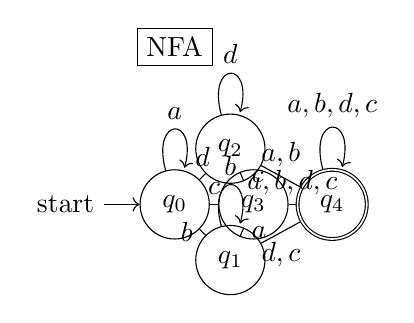
\begin{tikzpicture}
			\node[draw] at (0,2) {NFA};
			\node[state, initial] (q0) {$q_0$};
			\node[state, below right of=q0] (q1) {$q_1$};
			\node[state, above right of=q0] (q2) {$q_2$};
			\node[state, right of=q0] (q3) {$q_3$};
			\node[state, accepting, right of=q3] (q4) {$q_4$};
			\draw (q0) edge[loop above] node{$a$} (q0)
			(q0) edge[right,above] node{$c$} (q3)
			(q0) edge[left] node{$b$} (q1)
			(q0) edge[right, above] node{$d$} (q2)
			(q1) edge[loop above] node{$b$} (q1)
			(q1) edge[right] node{$a$} (q3)
			(q1) edge[below] node{$d,c$} (q4)
			(q2) edge[loop above] node{$d$} (q1)
			(q2) edge[right] node{$c$} (q3)
			(q2) edge[above ] node{$a,b$} (q4)
			(q3) edge[above] node{$a,b,d,c$} (q4)
			(q4) edge[loop above] node{$a,b,d,c$} (q4)
			;
		\end{tikzpicture}
	}
	\scalebox{.7}[.7]{
		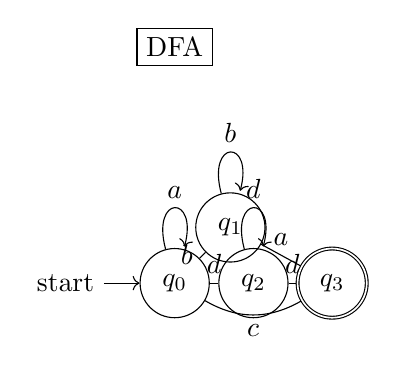
\begin{tikzpicture}
			\node[draw] at (0,3) {DFA};
			\node[state, initial] (q0) {$q_0$};
			\node[state, above right of=q0] (q1) {$q_1$};
			\node[state, right of=q0] (q2) {$q_2$};
			\node[state, accepting, right of=q2] (q3) {$q_3$};
			\draw (q0) edge[loop above] node{$a$} (q0)
			(q0) edge[bend right,below] node{$c$} (q3)
			(q0) edge[left] node{$b$} (q1)
			(q1) edge[loop above] node{$b$} (q1)
			(q2) edge[loop above] node{$d$} (q1)
			(q1) edge[above] node{$a$} (q3)
			(q0) edge[right, above] node{$d$} (q2)
			(q2) edge[right, above] node{$d$} (q3)
			;
		\end{tikzpicture}
	}
	\caption{NFA and DFA for regular expression \texttt{a*(b+a|d*c)}, autor's own work}
	\label{fig:regex_FSA}
\end{figure}
\subsubsection{Automata processing} \label{Automata processing}
The regular expression's matching process is equivalent to a finite state machine traversal of the input stream.
The process of matching begins with the activation of the initial states. Symbols from the input stream are sequentially utilized by the finite automaton.The process concludes once all the symbols of the input stream are processed.The incoming symbol is matched with the active states, and if it falls within the matchset of an active state, the active state transforms into a matched state ~\cite{Liu:Asynchronous}.

We can guarantee worst-case performance by restricting the processing of each input character. Techniques to limit per-character processing involve enlarging the finite automaton. Therefore, the search space is determined by balancing the size of the automaton and the upper limit of per-character processing~\cite{Nourian:DemystifyingFSA}.

\subsection{Graphics Processing Unit} \label{GPU}
The GPU, or Graphics Processing Unit, offers significantly higher instruction throughput and memory bandwidth than the CPU at a comparable price and power consumption.
While the CPU is optimized for rapid execution of a sequence of operations referred to as a "thread" and can execute dozens of these threads concurrently, the GPU is optimized for thousands of parallel executions (offsetting the slower single-thread performance for increased throughput).This variation in capabilities is a result of differing design objectives for the GPU and CPU.\footnote{From \url{https://docs.nvidia.com/cuda/cuda-c-programming-guide/index.html}}

All threads within a compute unit share a common instruction counter. Execution of a single compute unit occurs in lock-step, whereby each thread executes the same instruction when directed to do so. When control flow divergence occurs between threads within the same work group, divergent instructions are serialised,which can negatively impact performance.
Similarly, an unbalanced workload across threads in a work-group will result in idle threads, which reduces performance~\cite{yaneva2022gpuaccelerationFSA}.

The memory hierarchy of GPUs comprises: Global memory, a larger and slower form of memory accessible by all threads in any compute units. Constant memory, a read-only section of the global memory with a specific cache for faster memory access. Local memory, connected to compute units and shared among threads in a single unit and private memory, exclusively reserved for individual threads~\cite{yaneva2022gpuaccelerationFSA}.

\subsubsection{Parallel computing platforms} \label{Parallel computing platforms}
Due to the significant performance potential of GPUs, their  utilization has evolved from high-level shading languages to modern programming languages, reducing time and complexity involved in creating GPU-enabled applications~\cite{Asaduzzaman:Impact_CUDA_OpenCL}.
Two of the most popular APIs for GPU programming are CUDA\footnote{\url{https://developer.nvidia.com/cuda-toolkit}} (Compute Unified Device Architecture) and OpenCL\footnote{\url{https://www.khronos.org/opencl/}} (Open Computing Language). CUDA is a proprietary API developed by NVIDIA, while OpenCL is s an open royalty-free standard developed by the Khronos Group (an open, member-driven consortium, publishing and maintaining open standarts) \footnote{\url{https://www.khronos.org/}}.

OpenCL provides an efficient and portable way to access the power of different computing platforms. However, when comparing OpenCL to CUDA, there are sometimes performance differences. These differences are often attributed to the portability of OpenCL, which can lead to performance degradation. However, in a fair comparison, there is no inherent reason for OpenCL to perform worse than CUDA. Performance differences are primarily due to programmers and compilers behaviour\cite{Fang:Comparison-cuda-opencl}.

\section{Related Work} \label{Related work}
Research into the use of GPUs for regular expression matching started with the publications "Fast Exact String Matching on the GPU"\cite{schatz2007fast} and "A GPU-based Multiple-pattern Matching Algorithm for Network Intrusion
Detection Systems"\cite{huang2008gpu}. Their pioneering studies introduced a string matching program and multiple-pattern matching algorithm designed to take advantage of GPU processing capabilities.
This work was soon followed by "Accelerating Regular Expression Matching Using Hierarchical Parallel Machines on GPU"\cite{Lin:regex_gpu_parallel} and "GPU-based NFA Implementation for Memory Efficient High Speed Regular Expression Matching"\cite{Zu:GPU-NFA}. These two studies provide solutions to the performance challenges linked to regular expression matching in the context of network intrusion detection and other network functions.

Afterwards, a large, comprehensive study entitled "GPU Acceleration of Regular Expression Matching for Large Datasets: Exploring the Implementation Space"\cite{Becchi:regex_large_dataset} was published. The study examines regular expression matching on GPUs, focusing on practical-sized and complex datasets. It explores the advantages and limitations of different automata representations and various GPU implementation techniques.

Later, studies were published dealing with speeding up the processing of finite state machines. Papers "Scaling Out Speculative Execution of Finite-State Machines with Parallel Merge"\cite{Xia:FSA-scaling} and "On-the-Fly Principled Speculation for FSM Parallelization"\cite{zhao2015fly} introduce a speculative execution technique for finite state machines. "Why GPUs are Slow at Executing NFAs and How to Make them Faster"\cite{Liu:WhyGPUSlowNFA} proposed and evaluated optimisations to improve the throughput of NFA processing on GPUs by addresing tackle suboptimal data movement and underutilisation.
"Asynchronous Automata Processing on GPUs"\cite{Liu:Asynchronous} have developed a lightweight approach to increase the parallelism of automata processing on GPUs by asynchronously searching for patterns in the input stream in parallel.
\marginpar{GPU acceleration of finite state machine input execution:
	Improving scale and performance.
	nieco o CUDA/OPENCL}

\section{Objective and methodology} \label{Objective}

\section{Analysis} \label{Analysis}

\section{Results and discussion} \label{Results}

\section{Conclusions} \label{Conclusions} % prípadne iný variant názvu


\bibliography{zdroje}
\bibliographystyle{abbrv} % prípadne alpha, abbrv alebo hociktorý iný
\end{document}
